\chapter{実装}
\label{chap:implementation}

% \section{めも}

% Linuxカーネルのバージョン,System.mapの情報およびconfigの情報を知らなければ,メモリのみから正しくコンテキストを復元していくことはできない.

% libtlpの論文(もうちょっとちゃんと書く)で紹介されているprocess-list.cはSystem.mapを引数として渡し,
% \verb|init_task|の行をreadすることでinit_taskの仮想アドレスを得ている.
% また,カーネルコンフィグに依存するマクロの値や,使用する関数などもハードコーディングされており,論文の環境以外で動かすことが容易ではない.

\section{実装の概要}

本研究では,RDMAを用いて,動作中のマシンのメモリの値を取得していくことで,リモートホストから監視対象ホストのオペレーティングシステムのコンテキストを復元していくことを目指す.
この目的を実現するために,本研究では,NetTLP\cite{246316}を用いて実験を行う.

\section{NetTLP}
\label{section:nettlp}

NetTLPの目的は,PCIeデバイスの開発プラットフォームである.

その機能の一つとして,DMA messageとethernetパケットを相互変換する機能がある.
\ref{chap:related_works}で述べたが,RDMAのInfiniband実装は,制限が多い.(もう少し詳しく(3章に詳しく書く))
NetTLPにおけるRDMAでは,物理アドレスを指定することで,1Byteから4096Byteまでの任意のバイト数の値を取得することが可能である.
また,NetTLPを用いたRDMAでは,メインメモリの全メモリアドレスにアクセスすることが可能であり,アクセスできないメモリアドレスは存在しない,
すなわち全メモリアドレス空間から値を取得することが可能となっている.

NetTLPはFPGAボード上で動作するものであり,これを利用するためのインターフェースとして,libtlpが用意されている.
libtlpでは,RDMAを用いてメモリダンプを取得するためのインターフェースが関数として用意されている.
この関数を含んだヘッダファイルをincludeし,プログラムから呼び出すことで,メモリアドレスの値が返ってくる.

用意されている関数は,\verb|dma_read|関数と\verb|dma_write|関数の二つである.
\verb|dma_read|関数は,値を読みだすための関数であり,呼び出す際に読みたいメモリアドレスを渡す.
\verb|dma_write|関数は,値を指定した物理アドレスに書き込むための関数であり,呼び出す際に,書き込みたいメモリアドレスと値を渡す.

本研究では,\verb|dma_read|関数のみを用いる.

\subsection{process-list.c}

このファイルでやっていることをかく.
本研究の実装が,このprocess-list.cを拡張したものであるということを書く.

\section{実験環境}

本研究で実装を行う環境は,図\ref{fig:zentai}にあるように,NetTLP Adapterが書き込まれたFPGAが刺さった監視対象ホストと,本研究における実装を実行するホストの2台で構成する.

監視対象ホストは,Linux 4.15.0-72-genericのubuntuであり,PCIeデバイスとして,NetTLPが書き込まれたFPGAボードが刺さっている.
本研究では,FPGAボードとして,ザイリンクスのやつを使用している.(要加筆)
また,このFPGAボードは,ネットワークインターフェースでもあり,本研究の実験環境では,IPアドレスとして,192.168.10.1を静的に振ってある.

実装を実行するホストは,Linux 4.19.0-6-amd64のDebian busterであり,光ファイバーケーブル(名称はあとで修正)が刺さるNICを刺している.以後,実装ホストと呼称する.
このNICにはIPアドレスとして,192.168.10.3を静的に振ってある.
監視対象ホストに対してRDMAを実行する際は,\verb|dma_read|関数,あるいは\verb|dma_wirte|関数を通して192.168.10.1に対してIPパケットを送信する.

\begin{figure}[htbp]
    \caption{全体}
    \label{fig:zentai}
    \begin{center}
        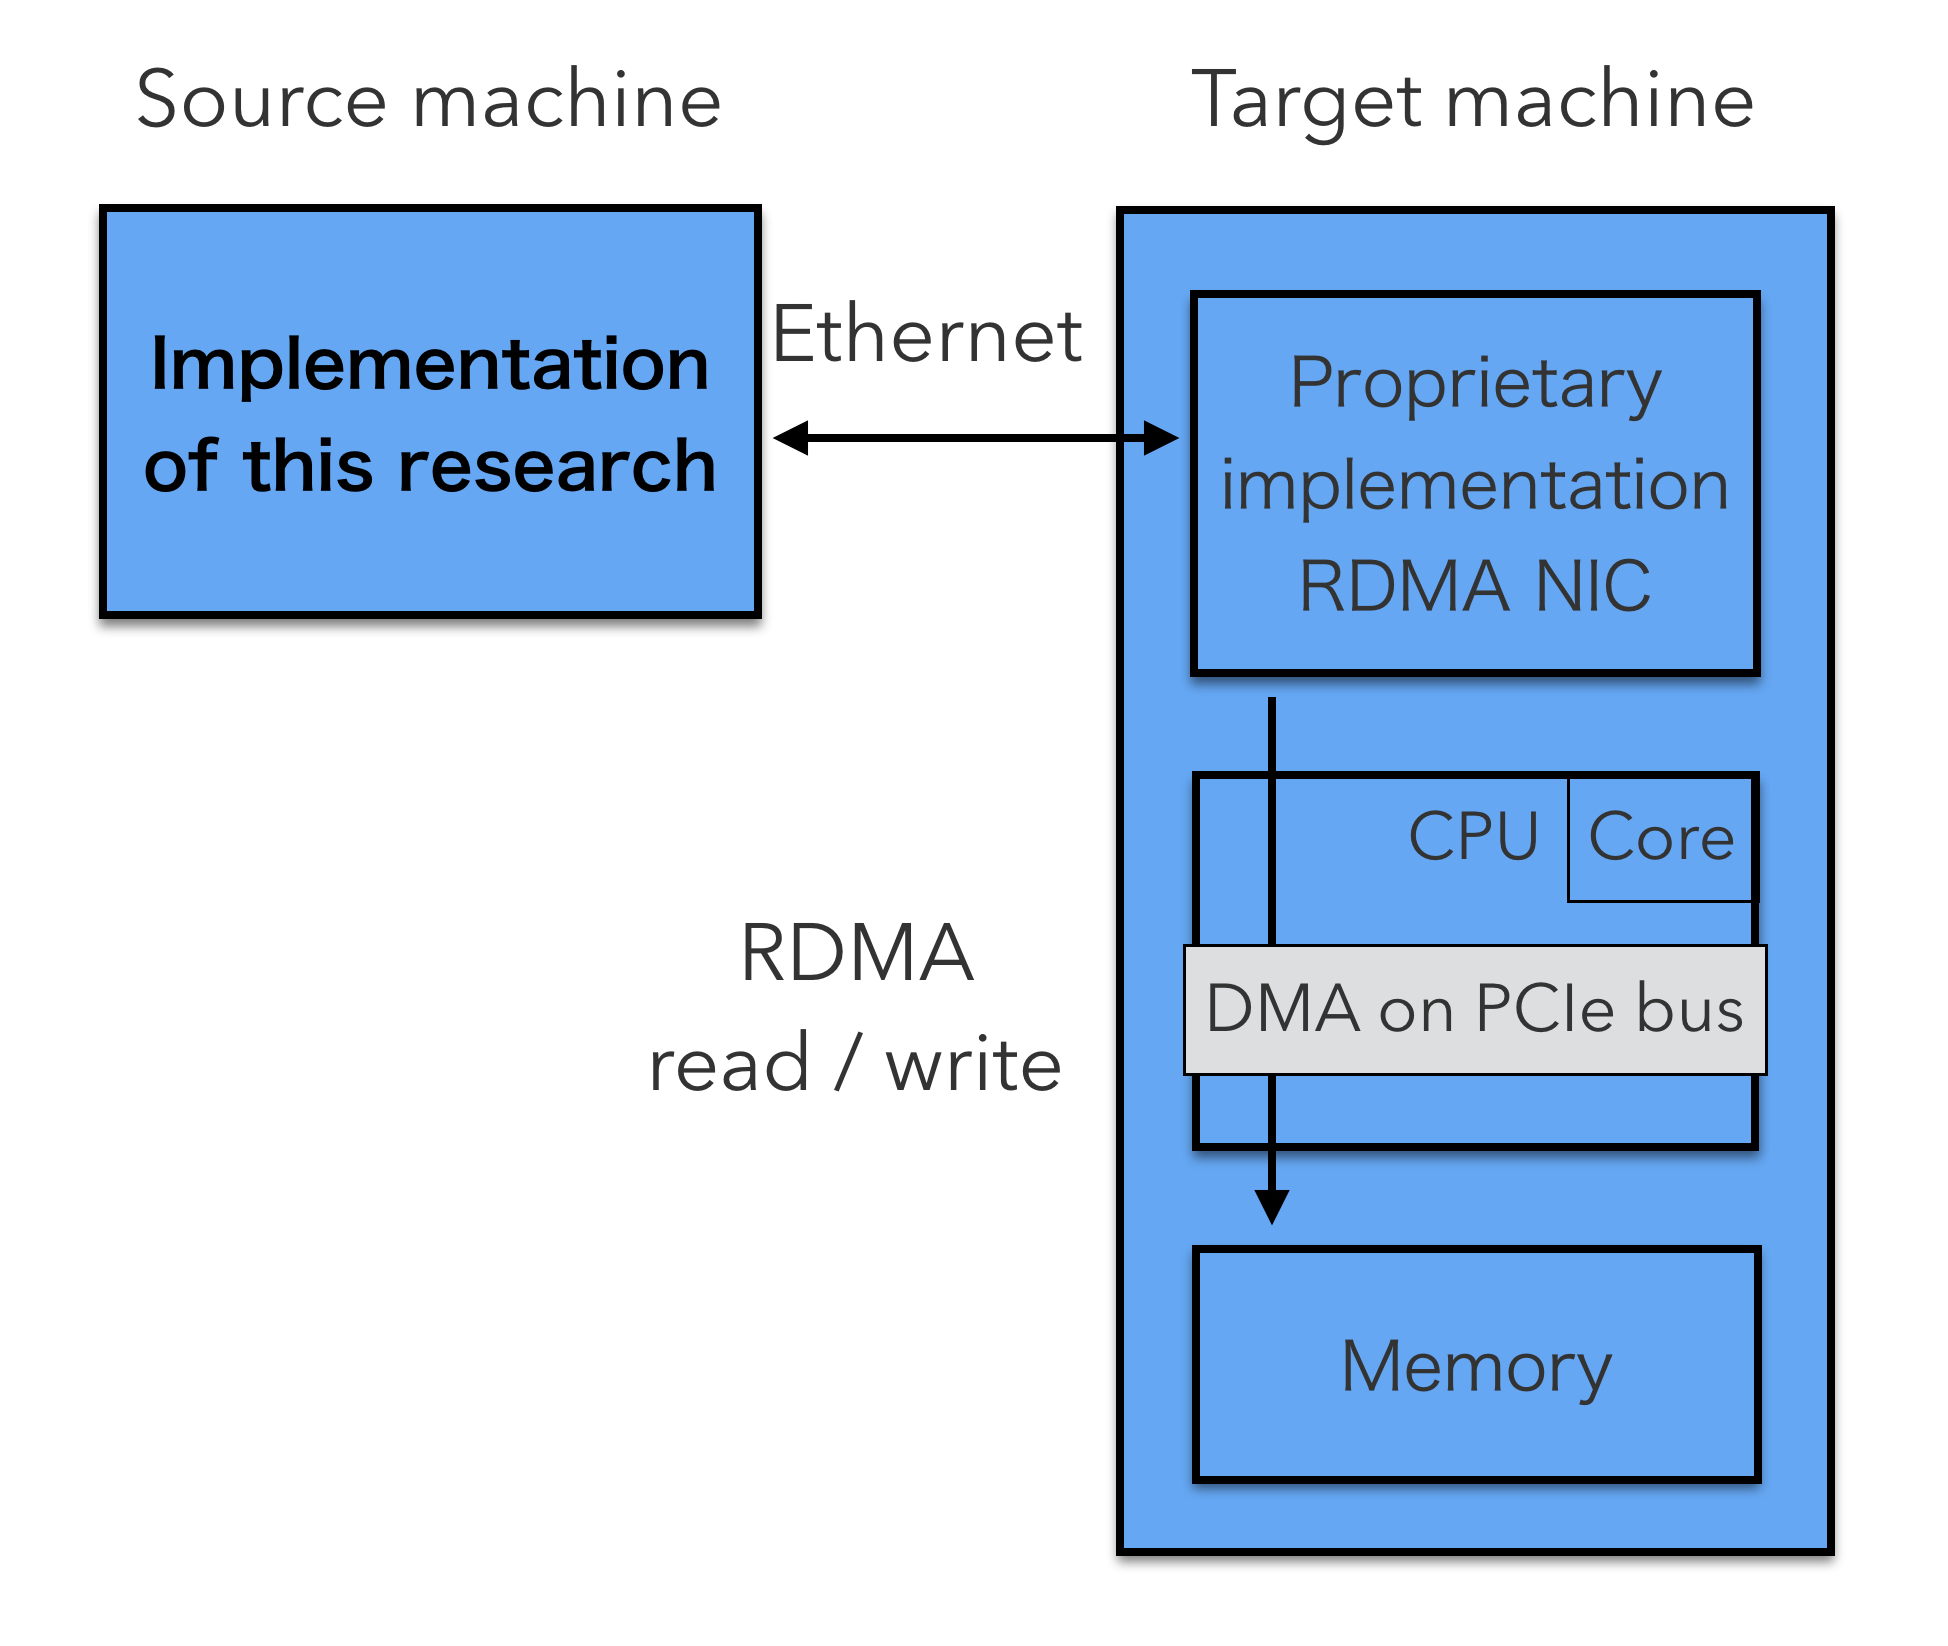
\includegraphics[bb=0 0 1000 800,width=15cm]{img/zentai.png}
    \end{center}
\end{figure}

\section{実装の前提情報}

本研究では,\ref{chap:approach}章で述べたように,
動作中のコンピュータのメインメモリの値を読むことによって監視対象ホストにおけるオペレーティングシステムのコンテキストを復元することを目的としている.
その手法として,RDMA NICを物理的に設置することで,この目的を達成することを試みている.

そこで,本研究の実装側のホストに与える情報を少なくすることが必要となる.
本セクションでは,本研究の実験において,実装を実行するホストが持っている情報と,初期段階では持っていないが解析の結果導き出す情報を分類する.

\ref{chap:approach}章で述べたように,オペレーティングシステムのコンテキストの復元,
その中でもLinuxにおいてプロセス情報の一覧を出すために必要な情報は以下の三点である.

一点目は,init_taskという,pidが0のプロセスのtask_struct構造体の開始アドレスである.
init_taskはコンピュータが起動する際に最初に実行されるプロセスであり,全てのプロセスは親プロセスを辿っていくことで,このプロセスにたどり着くことができる.
この情報は,実験に際して実装を実行するホストは,知らないこととする.(いいのか?)

二点目は,task_struct構造体の各フィールドの有無である.
Linuxカーネルでは,ビルドする際に,数千に及ぶ設定を記述し,マクロとして設定される.
この設定,kconfigによってtask_structは,どのフィールドを有効にするか,マクロとして定義された構造体の実体は何になるのか,などが決まる.
kconfigの結果によって,フィールドが存在するか否か,またそのフィールドが先頭アドレスからどのくらいのオフセットを持った状態で保持されているかが決まる.
すなわち,kconfigの情報によって,task_structのサイズや各フィールドの先頭アドレスからのオフセットが確定する.
このkconfigに関する情報は実験に際して実装を実行するホストは知らないこととする.

三点目は,Linuxカーネルのバージョンに関する情報である.
本研究では,実験する際に,監視対象ホストのカーネルのバージョンと同じソースコードを使用した上で実験を行う.
当然,Linuxカーネルのバージョンに関する情報は知っている必要がある.
Linuxカーネルのバージョンは,実装ホストは持っている情報とする.
\ref{section:want}で述べたもののうち,Linuxカーネルのバージョンは通知することとする

また,KASLR(kernel address space layout randomization)を無効にしてある.理由については,\ref{subsection:kaslr}にて述べる.

\subsection{KASLR}
\label{subsection:kaslr}

KASLRの簡単な説明と,無効にする理由と無効にしても良い理由を書く.

KASLRとは,kernel address space layout randomizationの略であり,カーネル領域における仮想アドレス空間のランダム化に関する仕組みのことである.
基本的な仕組みは,カーネルに限らず,プロセスの仮想アドレス空間のランダム化を実現する,ASLR(address space layout randomization)がある.
ASLRでは,実行ファイル内に存在するコードセグメントの仮想アドレスを,プロセスの実行のたびにランダムにする.

% todo: あれ,どのセグメントだっけ
ASLRが無効な状態でプロセスを実行すると,コードセグメントなどが常に一定の仮想アドレス空間にロードされるため,攻撃者にとって,仮想アドレスの推測が容易になってしまう.
これを防ぐための機構がASLRである.

KASLRでは,この考え方をカーネルの起動時にも適用するようにしたものである.

% todo: ここに説明を加筆

KASLRは,本研究においては,有効にしてもいい.ちょっと待て.

\section{実装の全体}

ダンプしてくるということを書く.物理アドレスのマッピングに関しても書く

実験における第一段階として,\ref{section:want}で述べたように,監視対象ホストのカーネルコンフィグおよび\verb|init_task|の先頭アドレスの仮想アドレスを知ることを目指す.
そこで,本研究では,この情報をメモリ上から探す.\ref{section:mem_dump}で述べる実装では,取得できるメモリダンプを全て取得し,解析する手法に関して述べる.

第二段階として,与えられたLinuxカーネルのバージョンのソースコードより,カーネルコンフィグの一覧を抽出し,その文字列を取得したメモリダンプから文字列探索をする.
文字列探索の結果取得したカーネルコンフィグの値をパースし,メモリ上から監視対象ホストのカーネルコンフィグを復元する.
\ref{section:restore_kconfig}で述べる実装では,カーネルコンフィグを復元する際の実装の詳細に関して記述する.

第三段階として,収集したカーネルコンフィグを元に手元のコンピュータでLinuxカーネルのソースコードに対してプリプロセスの処理を行い,\verb|task_struct|型を確定する.
また,\ref{section:approach}で述べた,監視対象ホストで動いているプロセスの一覧情報を取得するための
さらに,ソースコード上にある\verb|__phys_addr|関数の実体を収集する.

最後に,この工程で得られた情報をもとに,libtlpで提唱されている手法を用いて,プロセスの一覧を正しく取得できることを確認する.

\section{mem\_dump.c}
\label{section:mem_dump}

第一の工程として,メモリの全ての情報を取得する.ソースコードは以下である.この実装を実装ホストで実行し,出力結果をファイルに格納する.
この実装では,libtlpを通して,監視対象ホストのメモリを全探索する.この実装の実行には長い時間(何分?)かかるため,アトミックな情報ではない.
そのため,ここで取得したメモリダンプは,解析には使えない.
ここで取得したメモリダンプは,System.mapのうち,\verb|init_task|が配置されている仮想アドレス空間に関する情報および,Linuxカーネル 4.15.0におけるカーネルコンフィグに関する情報を収集するためのものである.

% Linuxカーネルにおける\verb|__phys_addr|関数,\verb|task_struct|型を決定するためのカーネルコンフィグに関する情報を収集することは\ref{chap:related_works}章で述べた.

\begin{itembox}[l]{実行方法}
    \begin{verbatim}
        ./dump_mem > ~/Desktop/work9/dump
    \end{verbatim}
\end{itembox}

\begin{itembox}[l]{mem_dump.c}
    \begin{verbatim}
        ここにソースを貼り付ける.
    \end{verbatim}
\end{itembox}

\section{カーネルコンフィグの復元}
\label{section:restore_kconfig}

Linuxカーネル4.15.0におけるカーネルコンフィグの一覧は,下に示す通りである(あとではるかも)

これらのコンフィグに関する情報を以下のスクリプトで読み出す.

カーネルコンフィグには,各設定項目に対する値として,y,mや文字列,数値などがあり,設定しない項目については,その行がコメント行になるのに加えて,\verb|is not set|という文言が付け足される.
これらの特徴を踏まえ,本研究では,restore_kconfig.pyというスクリプトをPythonを用いて実装した.
このスクリプトでは,得られたメモリダンプから,stringsコマンドを用いて文字列を抽出し,そこからkconfigの特徴である,CONFIGという文字列を含む行をgrepコマンドを用いて抽出する.
実行するシェルスクリプトは以下である.

\begin{itembox}[l]{strings}
    \begin{verbatim}
        strings dump | grep CONFIG > str_list
    \end{verbatim}
\end{itembox}

生成されたファイルに対して,上述したスクリプトを実行し,ファイルに書き出す.ここでは書き出すファイル名をrestored_kconfigとする.

\begin{itembox}[l]{exec restore_kconfig.py}
    \begin{verbatim}
        python restore_kconfig.py str_list > restored_kconfig
    \end{verbatim}
\end{itembox}

\begin{itembox}[l]{search config script}
    \begin{verbatim}
        実装した
    \end{verbatim}
\end{itembox}

上述した処理によって得られたrestored_kconfigというファイルを,後述するビルド時にコンフィグとして利用する.

\section{Linuxカーネルをプリプロセッサに通す}
\label{section:preprocess}

この工程では,収集したカーネルコンフィグを元に手元のコンピュータでLinuxカーネルのソースコードに対してプリプロセスの処理を行い,\verb|task_struct|型,
および\verb|__phys_addr|関数など,\verb|process-list.c|の影響のあるソースコードを確定する.

また,pid 0のプロセスのtask_struct構造体の先頭アドレスを知るため,またそれぞれのフィールドの先頭アドレスからのオフセットを確定させるため,オフセットを得る処理を施す.

まずは,事前に知らされた情報であるLinuxカーネルのバージョンより,適合したカーネルを取得する.
本研究の実装においては,バージョンは,4.15.0-72-genericである.

このソースコードに対して,\ref{section:restore_kconfig}で生成したファイルをコンフィグとして埋め込む.

\begin{itembox}[l]{build Linux kernel}
    \begin{verbatim}
        cd /path/to/linux-source-4.15.0
        cp /path/to/restored_kconfig .config
    \end{verbatim}
\end{itembox}

また,この工程では,カーネルビルド時におけるtask_struct型をバイナリではなくテキストファイルとして取得する必要があるため,
マクロを適用した直後の状態,すなわちプリプロセッサに通した直後の状態を保存するため,ビルド時の設定に変更を加える.
Linuxカーネルにおいては,ビルド時にMakefileを使用するため,このファイルを編集する.
具体的には,Linuxカーネル,バージョン4.15.0-72-genericにおいては,Makefileの447行目付近に,\verb|-save-temps|オプションを以下のような形で設定する.

\begin{itembox}[l]{-save-tempsオプションの設定・変更前}
    \begin{verbatim}
        LINUXINCLUDE   += -Iubuntu/include $(if $(KBUILD_SRC),-I$(srctree)/ubuntu/include)

        KBUILD_AFLAGS   := -D__ASSEMBLY__
        KBUILD_CFLAGS   := -Wall -Wundef -Wstrict-prototypes -Wno-trigraphs \
                -fno-strict-aliasing -fno-common -fshort-wchar \
                -Werror-implicit-function-declaration \
                -Wno-format-security \
                -std=gnu89
        KBUILD_CPPFLAGS := -D__KERNEL__
        KBUILD_AFLAGS_KERNEL :=
        KBUILD_CFLAGS_KERNEL :=
        KBUILD_AFLAGS_MODULE  := -DMODULE
        KBUILD_CFLAGS_MODULE  := -DMODULE
        KBUILD_LDFLAGS_MODULE := -T $(srctree)/scripts/module-common.lds
    \end{verbatim}
\end{itembox}

\begin{itembox}[l]{-save-tempsオプションの設定・変更後}
    \begin{verbatim}
        LINUXINCLUDE   += -Iubuntu/include $(if $(KBUILD_SRC),-I$(srctree)/ubuntu/include)

        KBUILD_AFLAGS   := -D__ASSEMBLY__
        KBUILD_CFLAGS   := -Wall -Wundef -Wstrict-prototypes -Wno-trigraphs \
                -fno-strict-aliasing -fno-common -fshort-wchar \
                -Werror-implicit-function-declaration \
                -Wno-format-security \
                -std=gnu89

        KBUILD_CFLAGS += -save-temps=obj

        KBUILD_CPPFLAGS := -D__KERNEL__
        KBUILD_AFLAGS_KERNEL :=
        KBUILD_CFLAGS_KERNEL :=
        KBUILD_AFLAGS_MODULE  := -DMODULE
        KBUILD_CFLAGS_MODULE  := -DMODULE
        KBUILD_LDFLAGS_MODULE := -T $(srctree)/scripts/module-common.lds
    \end{verbatim}
\end{itembox}

設定ファイルを書き終わったらビルドを行う.

\begin{itembox}[l]{ビルド}
    \begin{verbatim}
        make -j10
    \end{verbatim}
\end{itembox}

\section{task_struct構造体の確定}

Linuxカーネルのビルドが完了すると,上述したMakefileのKBUILD_CFLAGSの設定によって,中間ファイルを含む巨大なディレクトリおよび,vmlinux,bzImageが作成される.
本研究では,このビルドされたbzImageは使用しない.

\subsection{init_taskの開始アドレスの算出}

\subsection{init\_taskに関する情報の復元}

\ref{section:mem_dump}で作成した\verb|str_list|に対して,\verb|init_task|に関する行をgrepコマンドを用いて探す.

\begin{itembox}[l]{init_taskを探す}
    \begin{verbatim}
        cat str_list | grep "D init_task"
        # ffffffff82413480 D init_task
    \end{verbatim}
\end{itembox}

\section{得られた構造体を元に,実行ファイルを生成}

ていうか実装をカーネルに埋め込めばいいのでは

\ref{section:preprocess}で得ることができたソースをもとに,process-listを改造したものに関する説明をここに書く

\section{実装のまとめ}

この章は,相当長くなるので,まとめを書く.
